\section{Auswertung}
\label{sec:Auswertung}

\subsection{Justage}
\label{subsec:Justage}
In den PMTs, den Kabeln und den  Diskriminatoren können bei einem Myonensignal auf beiden Seiten des Szintillators unterschiedliche Verzögerungen
enststehen, was dazu führen kann, dass die Koinzidenzschaltung kein Signal weitergibt.
Zur Vermeidung gibt es vor den Diskriminatoren justierbare Verzögerungsschaltungen. Um die Verzögerung richtig zu justieren wird diese variiert und in einem $\qty{40}{\second}$ Intervall
das Myonensstartsignal gemessen. In \autoref{fig:Verzoegerung} ist das Myonensstartsignal gegenüber der eingestellten Verzögerung aufgetragen.
\begin{figure}[H]
  \centering
  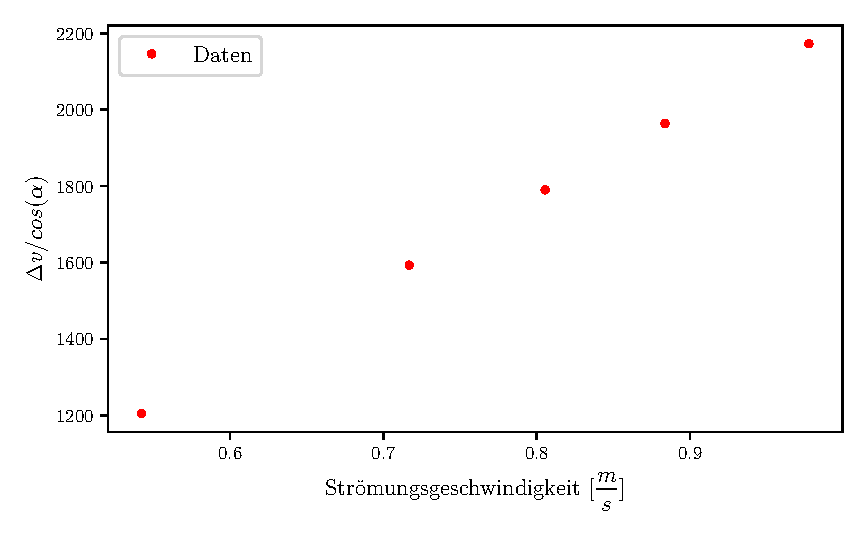
\includegraphics[width=\textwidth]{build/plot1.pdf}
  \caption {Messwerte der Justagemessung zur Bestimmung der Halbwertsbreite und der optimalen Verzögerung zwischen den beiden PMTs.}
  \label{fig:Verzoegerung}
\end{figure}
Der Graph zur Justierung der Verzögerungsleitungen in \autoref{fig:Verzoegerung} weist ein leichtes Plateau auf.
Dieses Plateau ist, wie in der Durchführung beschrieben, auf die normierte Pulsdauer der Ausgangssignale der Diskriminatoren zurückzuführen und befindet sich im erwarteten Bereich von \SI{10}{\nano \second}. \\
Zur Bestimmung der Halbwertsbreite wird zunächst die Höhe des Plateaus
\begin{align*}
    I_{Plateau} = (21.40 \pm 0.6) \si{\second^{-1}}
\end{align*}
berechnet, indem das arithmetische Mittel und Standardabweichung von dem Werten des Plateaus bestimmt wird.
Außerdem werden an beiden Seiten ein lineraer Fit eingefügt.
Die berchneten Parameter ergeben sich zu 
\begin{align}
  a_l &= (2.28 \pm 0.08)  \si{\nano\second^{-1}\second^{-1}} & b_l &= (42.06 \pm 1.11) \si{\second^{-1}} \\
  a_r &= (-2.15 \pm 0.04) \si{\nano\second^{-1}\second^{-1}} & b_r &= (56.03 \pm 0.73) \si{\second^{-1}}.
\end{align}
Danach wird die Halbwertsbreite bestimmt, indem die Schnittpunkte der Hälfte der mittleren Höhe des Plateaus mit den beiden Fits an der Seite zu
\begin{align*}
   \Delta t = t_r - t_l = (34.8 \pm 0.8) \si{\nano\second}
\end{align*}
berechnet werden.
Außerdem wird der Schnittpunkt der beiden Ausgleichsgeraden berechnet.
Dieser liegt bei $\Delta t = \qty{3.15}{\nano\second}$, weshalb für die Messung der Lebensdauer der Myonen eine Verzögerung von $\qty{3}{\nano\second}$
vor dem rechten Diskriminator eingestellt wird.


\subsection{Kalibration}
\label{subsec:Kalibration}
Um den Vielkanalanalysator zu kalibrieren werden mit Hilfe eines Doppelimpuls-Generators Impulse
mit unterschiedlichem zeitlichem Abstand eingelesen. Die belegten Kanäle sind in \autoref{fig:plot2} dargestellt und gegen die Impulsabstände aufgetragen.
\begin{figure}[H]
  \centering
  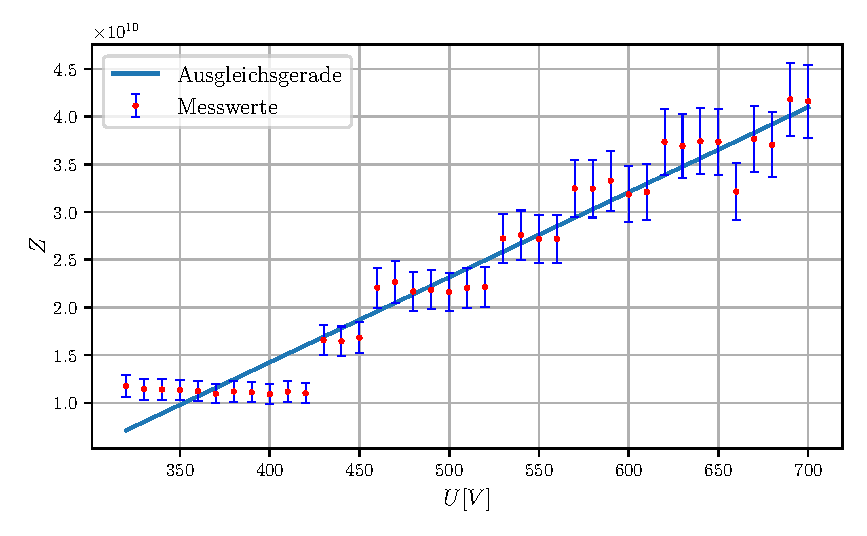
\includegraphics[width=0.7\textwidth]{build/plot2.pdf}
  \caption {Messwerte und Ausgleichsgerade der Kalibrationsmessung zur Umrechnung von Kanalnummern in Zerfallszeiten.}
  \label{fig:plot2}
\end{figure}
Außerdem wird ein linearer Fit angelegt. Die Beziehung zwischen der Zeit zwischen den Impulsen $\Delta t$ und der Kanalnummer lautet somit
\begin{align}
  \Delta t &= (\num{0.0217} \pm \num{1.35 e{-18}}) \si{\micro\second}  \cdot \text{Kanal}+ (\num{0.1304} \pm \num{3.43e-16})\si{\micro\second}.
  \label{eqn:tau}
\end{align}
Mithilfe dieser Funktion kann somit jedem Kanal eine Zeit zugeordnet werden.

\subsection{Berechnung des Untergrunds}
\label{subsec:Untergrund}

Bei der Messmethode, die in \autoref{subsec:Messmethode} beschrieben wird, kann es zu Messfehlern kommen, wenn in der eingestellten Suchzeit
\begin{align}
  T_S = \qty{10}{\micro\second}
  \label{eqn:Suchzeit}
\end{align}
ein weiteres Myon in den Tank eintrifft, was dann zu einem falschen Stoppsignal führt. 
Es tritt somit ein Untergrund über die gesamte Messzeit
\begin{align}
  T_{ges} = \qty{169832.86}{\second}
  \label{eqn:Messzeit}
\end{align}
auf, der sich gleichmäßig auf die Kanäle aufteilt, aufgrund der Unabhängigkeit der Myonen.
Die Wahrscheinlichkeit, dass $n$ Myonen bei einem Erwartungswert
\begin{align*}
  \mu(T_S) = I_{Mess} T_S
  \label{eqn:Erwartungswert}
\end{align*}
in der Zeit $T_S$ in den Detektor einfallen ist poissonverteilt
\begin{equation}
  p_{\mu} = \frac{\mu}{n!} \text{e}^{-\mu}.\label{eqn:Poission}
\end{equation}
Die durchschnittlich gemessene Rate $I_{Mess}$ lässt sich mit
\begin{align*}
  I_{Mess} = \frac{N_{Start}}{T_{ges}} = \qty{27.95 \pm 0.01}{\second\tothe{-1}}
\end{align*}
berechnen, wobei $N_{Start}$ die gesamt Anzahl der Startimpulse 
\begin{align*}
  N_{Start} = \qty{4747339 \pm 2178.84}{} 
\end{align*}
ist.
Der gesamte Untergrund ergibt sich nun aus \autoref{eqn:Poission} für ein Teilchen $(n=1)$ und der Anzahl der Startimpulse zu
\begin{align}
  U_{ges} = p_{\mu}(1) N_{Start} = \num{1326.70 \pm 1.20}.
\end{align}
Dieser Untergrund muss nun auf die relevanten Kanäle normiert werden. Dabei beträgt die Anzahl der relevanten Kanäle in $T_S$ $435$ und somit ergibt sich der Untergrund zu
\begin{align}
  U_n = \frac{U_{ges}}{435} = \num{3.050 \pm 0.003}.
\end{align}

\subsection{Lebenszeit der Myonen}
\label{subsec:Lebenszeit}
Die vom Vielkanalanalysator aufgenommenen Messwerte für die Counts pro Kanal sind in \autoref{fig:plot3} dargestellt.
\begin{figure}[H]
  \centering
  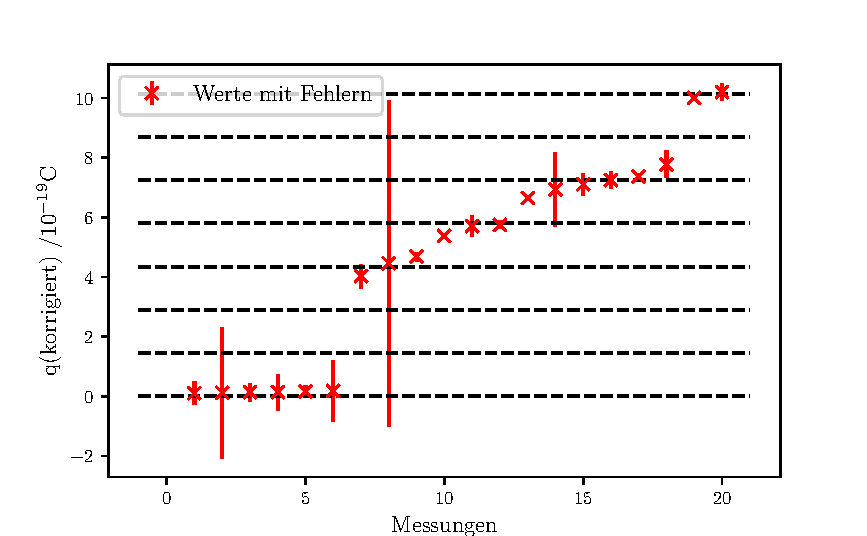
\includegraphics[width=\textwidth]{build/plot3.pdf}
  \caption {Um den Untergrund korrigierte Messwerte der Lebensdauer-Messung und Exponentialfit.}
  \label{fig:plot3}
\end{figure}

Hierbei wurde von den aufgenommenen Daten schon der in \autoref{subsec:Untergrund} berechnete Untergrund abgezogen.
Ein Exponentialfit der Form
\begin{align*}
  N(t) &= N_0 \cdot \exp(-t \mathbin{/} \text{Kanal})
\end{align*}
mit den Parametern 
\begin{align*}
  N_0 &= (156.1 \pm 1.2)\\
  \text{Kanal} &= (93.4 \pm 1.0)
\end{align*}
ist außerdem dargestellt.
Hierbei werden die ersten Werte außer Acht gelassen, da sie nicht dem exponentiellen Verlauf folgen.
Somit kann mithilfe von \autoref{eqn:tau} der Abstand der Impulse, beziehungsweise die mittlere Lebensdauer der kosmischen Myonen
zu 
\begin{align*}
  \tau &= (2.160 \pm 0.021)\si{\micro\second}
\end{align*}
bestimmt werden.

